%************************************************
\chapter{Preliminaries}\label{ch:prelim}
%************************************************

The goal of this chapter is to provide a formal background on the covered material, together with a unified notation (which differs quite a lot from publication to publication). After we establish some basic theoretical foundations in \secref{prelim:essentials}, we remind the reader of the basic notions of reinforcement learning in \secref{prelim:rl} and of the recently explored and useful distributional reinforcement learning in \secref{prelim:distrl}. We follow up with the basics of risk together with the crucial CVaR measure in \secref{prelim:risk}.

The interested reader is welcome to explore the books and publications referenced throughout this chapter and in \secref{prelim:literature}. An informed reader may choose to skip to \secref{prelim:problem} where we formalize the problems tackled in this thesis.

\section{Probability Essentials}\label{sec:prelim:essentials}

random variable

exp value


\todo{operator contraction}



%***********************************************************************************************************************************************************
%***********************************************************************************************************************************************************
%***********************************************************************************************************************************************************


\section{Reinforcement Learning}\label{sec:prelim:rl}

The idea that we learn by interacting with our environment is probably the first to occur to us when we think about the nature of learning. Reinforcement learning \cite{sutton1998reinforcement} is a sub-field of machine learning that deals with time-dependent decision making in an unknown environment. The learner (often called agent) is not told which actions to take, but instead must discover which actions yield the most reward by trying them. In the most interesting and challenging cases, actions may affect not only the immediate reward but also subsequent situations and rewards. These two characteristics, trial-and-error search and delayed reward are the most important distinguishing features of reinforcement learning.

The general interaction between the agent and an environment can be seen in \figref{prelim:rlloop}. In each time-step $t$, the agent receives an observation $x_t$ and a reward $r_t$ and picks an action $a_t$ and the process repeats. Below we formalize all the necessary notions of states and actions as a Markov Decision Process.

\begin{figure}[h]
\center
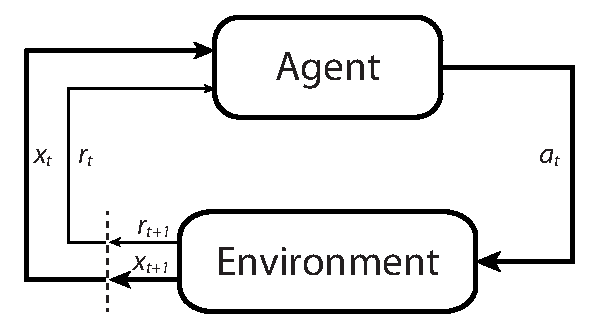
\includegraphics[width=.6\linewidth]{gfx/rl_loop.pdf}
\caption{The Reinforcement learning cycle}
\label{fig:prelim:rlloop}
\end{figure}

\subsection{Markov Decision Processes}

Markov Decision Process (MDP, \citet{bellman1957markovian}) is a classical formalization of sequential decision making, where actions influence not just immediate rewards, but also subsequent situations, or states, and through those future rewards. They are a mathematically idealized form of the reinforcement learning problem for which precise theoretical statements can be made.

The word Markov points to the fact that we assume that the state transitions of an MDP satisfy the Markov property \cite{???}. This means that the conditional probability distribution of future states of the process depends only upon the present state and not the whole history of events that preceded it.

\begin{definition}

MDP is a 5-tuple $\mathcal{M} = (\cX, \cA, R, P, \gamma)$, where 

$\cX$ is the finite state space

$\cA$ is the finite action space

$R(x, a) \in [R_{\min}, R_{\max}]$ is a random variable representing the reward generated by being in state $x$ and selecting action $a$

$P(\cdot|x, a)$ is the transition probability distribution

$\gamma \in [0, 1)$ is a discount factor
\end{definition}

\begin{definition}
A stationary (or markovian) policy is a mapping from states to actions $\pi:\cX \to \cA$.
\end{definition}

When solving MDPs with the usual discounted expected value criterion, it is common to limit the policy space to stationary policies, where the decision to take an action depends only on the current state. Unfortunately, when one considers other more general criteria, it is necessary to consider the whole action-state history that led up to the last state. This fact leads to the definition of a history-dependent policies.

\todo{make the following readable}
\begin{definition}
Let the space of admissible histories up to time $t$ be $H_t = H_{t-1} \times \cA \times \cX$ for $t \ge 1$, and $H_0 = \cX$. A generic element $h_t \in H_t$ is of the form $h_t = (x_0, a_0, ..., x_{t-1}, a_{t-1})$. Let $\Pi_{H,t}$ be the set of all history-dependent policies with the property that at each time $t$ the randomized control action is a function of $h_t$. In other words, 
$\Pi_{H,t} = \mathbb{R}aces{\pi_0: H_0 \to \mathbb{P}(\cA), ..., \pi_t: H_t \to \mathbb{P}(\cA)|\pi_i(h_i) \in \mathbb{P}(\cA) \forall h_i \in H_i, 1\le i\le t}$. We also let $\Pi_H = \lim_{t\to\infty}\Pi_{H,t}$ be the set of all history-dependent policies.
\end{definition}

\todo{as will become clear later, we can limit ourselves to an extended state spaces, not necessarily noting the whole history}

\subsection{Return}

The reinforcement learning framework, generally considers either the natural discounted infinite-horizon return \todo{few sentences on discounted/undiscounted returns}



We define the return $Z^\pi(x)$ as a random variable representing the discounted reward along a trajectory generated by the MDP by following the policy $\pi$, starting at state $x$

\begin{equation}
\begin{split}
Z^\pi(x)=\sum_{t=0}^\infty \gamma^tR(x_t,a_t)\\
x_t \sim p(\cdot|x_{t-1}, a_{t-1}), a_t \sim \pi, x_0 = x
\end{split}
\end{equation}

As a useful notation, we denote $Z^\pi(x, a)$ as the random variable representing the discounted reward along a trajectory generated by first selecting action $a$ and then following policy $\pi$.

\begin{equation}
\begin{split}
Z^\pi(x, a)=\sum_{t=0}^\infty \gamma^tR(x_t,a_t)\\
x_t \sim p(\cdot|x_{t-1}, a_{t-1}), a_t \sim \pi, x_0 = x, a_0 = a
\end{split}
\end{equation}

We will sometimes omit the superscript $\pi$ when the policy is clear from the context.

\subsection{Bellman equation}

The \textit{value function} $V^\pi$ of a policy $\pi$ describes the expected return received from state $x \in \cX$ and acting according to $\pi$:

\begin{equation}
\begin{split}
V^\pi(x) = \expect Z^\pi(x) = \expect\left[\sum_{t=0}^\infty \gamma^tR(x_t,a_t) \right]\\
x_t \sim p(\cdot|x_{t-1}, a_{t-1}), a_t \sim \pi, x_0 = x
\end{split}
\end{equation}


The \textit{action-value} function $Q^\pi$ of a policy $\pi$ describes the expected return from taking action $a \in \cA$ from state $x \in \cX$, then acting according to $\pi$:

\begin{equation}
\begin{split}
Q^\pi(x, a) = \expect Z^\pi(x, a) = \expect\left[ \sum_{t=0}^\infty \gamma^tR(x_t,a_t) \right]\\
x_t \sim p(\cdot|x_{t-1}, a_{t-1}), a_t \sim \pi, x_0 = x, a_0 = a
\end{split}
\end{equation}

Fundamental to reinforcement learning is the use of Bellman’s equation \citep{bellman1957markovian} to describe the value and action-value functions by a recursive relationship:

\begin{equation}
V^\pi(x) = \expect R(x, \pi(x)) + \gamma \expect\limits_{p, \pi}V^\pi(x')
\end{equation}

\begin{equation}
Q^\pi(x, a) = \expect R(x, a) + \gamma \expect_{p, \pi}V^\pi(x')
\end{equation}

In reinforcement learning we are typically interested in acting so as to maximize the expected return. The most common approach for doing so involves the optimality equation
\begin{equation*}
Q^*(x,a) = \expect R(x,a) + \gamma \expect\nolimits_p \max_{a' \in \cA} Q^*(x', a') .
\end{equation*}
This equation has a unique fixed point $Q^*$, the optimal value function, corresponding to the set of optimal policies $\Pi^*$ ($\pi^*$ is optimal if $\expect_{a \sim \pi^*} Q^*(x, a) = \max_a Q^*(x,a)$).

We view value functions as vectors in $\mathbb{R}^{\cX \times \cA}$, and the expected reward function as one such vector. In this context, the \emph{Bellman operator} $\cT^\pi$ and \emph{optimality operator} $\cT$ are
\begin{align}
\cT^\pi Q(x,a) &:= \expect R(x,a) + \gamma \expect_{P, \pi} Q(x',a')\\
\cT Q(x,a) &:= \expect R(x,a) + \gamma \expect_{P} \max_{a' \in \cA} Q(x', a')
\end{align}
These operators are useful as they describe the expected behaviour of popular learning algorithms such as SARSA and Q-Learning \cite{sutton1998reinforcement}. In particular they are both contraction mappings, and their repeated application to some initial $Q_0$ converges exponentially to $Q^\pi$ or $Q^*$, respectively \citep{bertsekas1995neuro}.


%***********************************************************************************************************************************************************
%***********************************************************************************************************************************************************
%***********************************************************************************************************************************************************


\section{Distributional Reinforcement Learning}\label{sec:prelim:distrl}

In contrast to standard reinforcement learning, where we model the expected value of the return, in distributional reinforcement learning \cite{many} we aim to model the full distribution of return. This is advantageous in cases where we want to e.g. model parametric uncertainty \cite{...} or design risk-sensitive algorithms \citep{morimura2012parametric}\citep{morimura2010nonparametric}. \citet{bellemare2017distributional} also argue, that the distributional approach is beneficial even in the case we are optimizing the expected value, as the distribution gives us more information which helps the now commonly used approximate algorithms (such as DQN \citep{mnih2015human}).

At the core of the distributional approach lies the recursive equation of the return distribution:

\begin{equation}
\begin{split}
Z(x, a) \overset{D}{=} R(x, a) + \gamma Z(x', a')\\
x_t \sim p(\cdot|x_{t-1}, a_{t-1}), a_t \sim \pi, x_0 = x, a_0 = a
\end{split}
\end{equation}

where $\overset{D}{=}$ denotes that random variables on both sides of the equation share the same probability distribution.

In the \emph{policy evaluation} setting \citep{sutton98reinforcement} we are interested in the value function $V^\pi$ associated with a given policy $\pi$. The analogue here is the value distribution $Z^\pi$. In this section we characterize $Z^\pi$ and study the behaviour of the policy evaluation operator $\cT^\pi$. Note that $Z^\pi$ describes the intrinsic randomness of the agent's interactions with its environment, rather than some measure of uncertainty about the environment itself.
%

We view the reward function as a random vector $R \in \mathcal{Z}$, and define the transition operator $P^\pi : \mathcal{Z} \to \mathcal{Z}$
%\begin{align}
%P^\pi Z(x, a) &\overset{D}{=} Z(X', A') \label{eqn:policy_operator} \\
%X' &\sim P(\cdot \cbar x, a), \, A' \sim \pi(\cdot | X'), \nonumber
%\end{align}
where we use capital letters to emphasize the random nature of the next state-action pair $(X', A')$.
We define the distributional Bellman operator $\cT^\pi : \mathcal{Z} \to \mathcal{Z}$ as
\begin{equation}
\cT^\pi Z(x,a) \overset{D}{=} R(x,a) + \gamma P^\pi Z(x,a).
\end{equation}

We emphasize that this is a distributional equation and the distributional bellman operator is therefore fundamentally different from the standard bellman operator.

\citet{bellemare2017distributional} have shown, that the distributional bellman operator $\cT^\pi$ is not a contraction in the commonly used KL divergence \cite{...}, but is a contraction in the infinity wasserstein metric which we describe bellow, as it will become useful as a tool for evaluating algorithms in the rest of the thesis. Another important fact is, that the bellman optimality operator $\cT$ is not a contraction in any metric \unclear{formally state this? would require more definitions}. The distribution does not converge to a fixed point, but rather to a sequence of optimal (in terms of expected value) policies.

\subsection{The Wasserstein Metric}
\newcommand{\pnorm}[1]{\| #1 \|_p}

One of the tools for analysis of distributional approaches to reinforcement learning is the Wasserstein metric $d_p$ between cumulative distribution functions \citep[see e.g.][where it is called the Mallows metric]{bickel81asymptotic}. For $F$, $G$ two c.d.fs over the reals, it is defined as
\begin{equation*}
d_p(F, G) := \inf_{U, V} \pnorm{U - V},
\end{equation*}
where the infimum is taken over all pairs of random variables $(U, V)$ with respective cumulative distributions $F$ and $G$. The infimum is attained by the inverse c.d.f. transform of a random variable $\mathcal{U}$ uniformly distributed on $[0, 1]$:
\begin{equation*}
d_p(F, G) = \| F^{-1}(\mathcal{U}) - G^{-1}(\mathcal{U}) \|_p .
\end{equation*}
For $p < \infty$ this is more explicitly written as
\begin{equation}
d_p(F, G) = \left ( \int_0^1 \big | F^{-1}(u) - G^{-1}(u) \big |^p du \right )^{1/p} .
\end{equation}

\todo{explain in words, also mention why it's better than KL}
\todo{maybe visuals, if it will become important}

%***********************************************************************************************************************************************************
%***********************************************************************************************************************************************************
%***********************************************************************************************************************************************************


\section{Risk-Sensitivity}\label{sec:prelim:risk}




\subsection{Value-at-Risk}

\todo{introduction, importance, flaws, ...}
Let $Z$ be a bounded-mean random variable, i.e. $\expect[|Z|] < \infty$, with cummulative distribution function (c.d.f.) $F(z) = \mathbb{P}(Z \le z)$.
In this paper we interpret $Z$ as a reward\footnote{This is in accordance with reinforcement learning literature and opposed to risk-related literature.}. The value-at-risk (VaR) at confidence level $\alpha \in (0,1)$ is the $\alpha$ quantile of $Z$, i.e. 

\begin{equation}
\text{VaR}_\alpha(Z)=F^{-1}(\alpha)=\max\left\lbrace z | F(z) \le \alpha \right\rbrace
\end{equation}

We will use the notation $\text{VaR}_\alpha(Z)$, $F^{-1}(\alpha)$ interchangebly, often explictly denoting the random variable of inverse c.d.f. as $F^{-1}_Z(\alpha)$.

\subsection{Conditional Value-at-Risk}
\todo{introduction, robustness, ...}
The conditional value-at-risk (CVaR) at confidence level $\alpha \in (0,1)$ is defined as:

\begin{equation}
\text{CVaR}_\alpha(Z) = \dfrac{1}{\alpha}\int_0^\alpha F^{-1}_Z(\beta) \text{d}\beta = \dfrac{1}{\alpha}\int_0^\alpha \text{VaR}_\beta(Z) \text{d}\beta
\end{equation}

We will also use the following equivalent formulation from \cite{rockafellar2000optimization}:

\begin{equation}\label{eq:cvardef}
\text{CVaR}_\alpha(Z)=
\max_s\left\lbrace \dfrac{1}{\alpha}\expect
\left[ (Z-s)^-\right] + s  \right\rbrace 
\end{equation}

where $(x)^- = \min(x, 0)$ represents the negative part of $x$.

\begin{figure}
\center
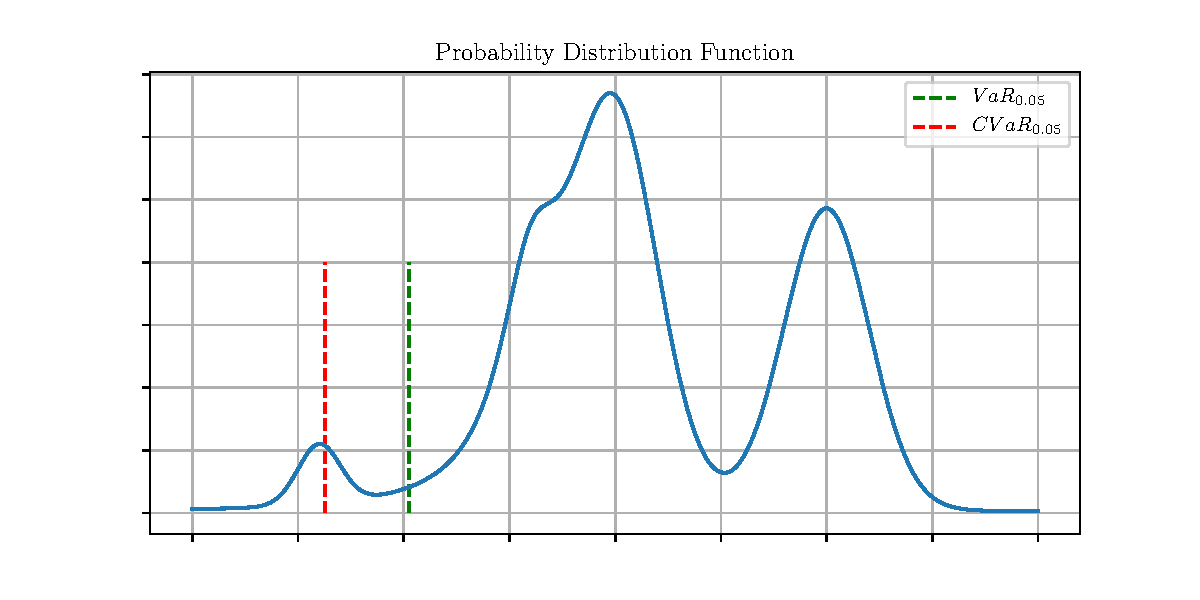
\includegraphics[width=\linewidth]{gfx/pdf.pdf}
\caption{Value-at-Risk and Conditional Value-at-Risk of a general probability distribution with $\alpha=0.05$. The main flaw of the VaR metric is clearly visible here, as we could shift the leftmost }
\end{figure}




%*****************************************
%*****************************************
%*****************************************

\section{Problem Formulation}\label{sec:prelim:problem}

\todo{combine rl and risk, remind motivations}


The risk-sensitive problem we wish to adress for a given confidence level $\alpha$ is as follows:
\begin{equation}
\max_\pi \text{CVaR}_\alpha(Z^\pi(x_0))
\end{equation}


\subsection{Time-consistency}
An important property of CVaR MDPs is that of time-consistency. ***Choose one definition, describe*** The notion of time consistency varies from author to author; in Shapiro [XXX] it is shown ***.

*** Policy gradient literature ignores the time consistency-issue, leading to locally optimal policies *** show that they can be worse than EXP ***.


%*****************************************
%*****************************************
%*****************************************

\section{Literature Survey}\label{sec:prelim:literature}


